\chapter{Theoretical Foundations}

After a short introduction to the terminology of Big Data, this chapter will discuss the main
characteristics of Big Data Analytics Applications and introduces the concept of stream processing,
which is one of the main characteristics of the popular streaming frameworks Apache Flink and
Apache Kafka. The underlying concepts both of these systems and how they're used in context of
Big Data Analytics will be explained at the end of this chapter.

\section{Big Data}

According to \cite{Marz15} the term “Big Data” is a misleading name since it implies that pre-existing
data is somehow small, which is not true, or that the only challenge is the sheer size of data, which
is just one one them among others. In reality, the term Big Data applies to information that can’t be
processed or analyzed using traditional processes or tools.

In the past decade the amount of data being created is a subject of immense growth. More than
30,000 gigabytes of data are generated every second, and the rate of data creation is only
accelerating.\cite{Marz15}. People create content like blog posts, tweets, social network interactions,
photos, servers continuously log messages, scientists create detailed measurements, permanently.

\begin{figure}[H]
	\centering
	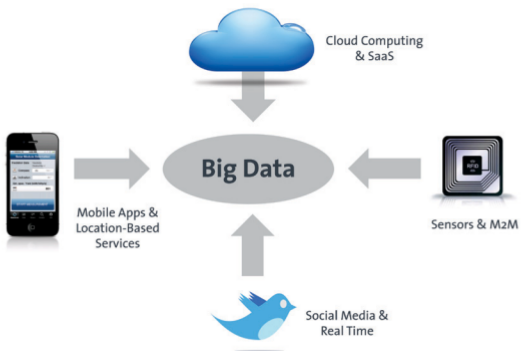
\includegraphics[width=0.7\textwidth]{../images/04-sources-of-bigdata.png}
	\caption{Sources of Big Data{\cite{Bitk12}}}
	\label{sources-of-bigdata}
\end{figure}

Through advances in communications technology, people and things are becoming increasingly interconnected.
Generally referred to as machine-to-machine (M2M), interconnectivity is responsible for double-digit year
over year (YoY) data growth rates. Finally, because small integrated components are now affordable, it
becomes possible to add intelligence to almost everything. As an example, a simple railway car has
hundreds of sensors for tracking the state of individual parts and GPS-based data for shipment tracking
and logistics.\cite{Ziko12}

Besides the extremely growing amount of data, an increase in data diversity goes hand in hand.
It comes in its raw and unstructured, semistructured or structured form, which makes processing it in a
traditional relational system impractical or impossible. In \cite{Bitk12} is described, that around
85 percent of the data comes in an unstructured form, but containing valuable information.

According to \cite{Marz15} \cite{Ziko12}, Big Data is defined by three characteristics:
\begin{description}
    \item [Volume] The amount of data present is growing because of growing amount of producers,
    e.g. environmental data, financial data, medical data, surveillance data.
    \item [Variety] Data varies in its form, it comes in different formats from different sources.
    \item [Velocity] Data needs to be evaluated and analyzed quickly, which leads to new challenges
    like analysis of large data sets with answers in seconds range, data processing in realtime,
    data generation and transmission at highspeed.
\end{description}
\begin{figure}[H]
	\centering
	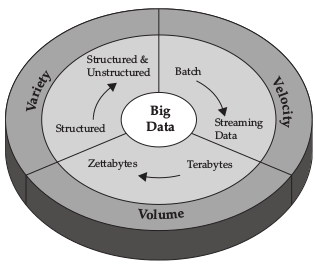
\includegraphics[width=0.7\textwidth]{../images/03-three-vs-of-bigdata.png}
	\caption{The three 'V's of Big Data{\cite{Ziko12}}}
	\label{three-vs-of-bigdata}
\end{figure}

A possible definition for Big Data could be derived as follows: \textit{Big Data refers to the use of
large amounts of data from multiple sources with a high processing speed for generating valuable information
based on the underlying data.}

\cite{Bitk12} adds another characteristic as a fourth point called "Analytics", which will be explained in the
next section.

\section{Big Data Analytics Applications}

Another definition comes from the the science historian George Dyson, who was cited by Tim O'Reilly in \cite{Dys13}:
\textit{Big data is what happened when the cost of storing information became less than the cost of making the
decision to throw it away.} It follows that the storage and extraction of valuable information from the immense amount of
existing data has become the most important part of Big Data Analytics Applications.

Big Data Analytics describes the process of collecting, organizing and analyzing large volumes
of data with the aim to discover patterns, relationships and other useful information extracted from incoming
data streams \cite{Marz15}. The process of analytics is typically performed using specialized software tools and
applications for predictive analytics, data mining, text mining, forecasting and data optimization.

The analytical methods raise data quality for unstructured data on a level that allows more quantitative and
qualitative analysis. With this structure it becomes posssible to extract the data that is relevant by iteratively
refined queries.

The areas of applications may be extremely diverse and ranges from analysis of financial flows or traffic data,
processing sensor data or environmental monitoring as explained in the previous chapter.

The illustration below summarises the six-dimensional taxonomy \cite{Bitk14, Csa14} of Big Data Analytics Applications,
which will be discussed in the following:
\begin{figure}[H]
	\centering
	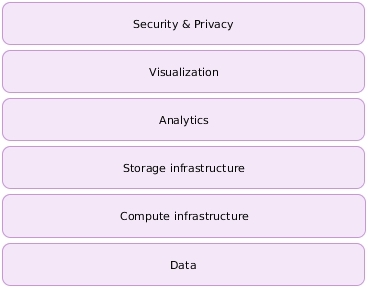
\includegraphics[width=0.7\textwidth]{../images/05-big-data-taxonomy.jpg}
	\caption{Taxonomy of Big Data Analytics Applications \cite{Bitk14, Csa14}}
	\label{taxonomy-bigdata-applications}
\end{figure}




\section{Stream Processing}
According to \cite{Klepp16}, stream processing is the real-time processing of data continuously,
concurrently, and in a record-by-record fashion in which data is treated not as static tables
or files, but as a continuous infinite stream of data integrated from both live and historical
sources.

Check \cite{Marz15} S.225 ff.


%If an application demands “immediate” response to each event as it occurs, some form of stream processing is needed,
%which essentially processesthe data as it comes in. The general approach is to have a little bit of code that processes
%each ofthe events separately. In order to speed up the processing, the stream may be subdivided, and the computation
%distributed across clusters.
%Apache Stormis a popular framework for event processing that was developed at Twitter and promulgated by Twitter
%and other companies that required this paradigm of real-time processing. Other examples are Amazon’s Kinesis, or the
%streaming capabilities of MapR. These frameworks take care of the scaling onto multiple cluster nodes and come with
%varying degrees of support for resilience and fault tolerance, for example, through checkpointing, to make sure the
%system can recover from failure.

%These stream processing frameworks primarily address only parallelization of the computational load; an additional
%storage layer is needed to store the results in order to be able to query them. While the “current state” of the
%computation is contained in the stream processing framework, there is usually no clean way to access or query this
%information, particularly from external modules. Depending on the amount of data that is being processed, this might
%further entail the need for a large, high-performance storage backend.
%Apache Spark (discussed in more detail below), simplistically speaking, takes a hybrid approach. Events are collected in a
%buffer and then processed at fixed intervals (say every few seconds) in a batch fashion. Since Spark holds the data in
%memory, it can in principle process the batches fast enough to keep up with the incoming data stream.
%In summary, low latency processing generally entails some form of stream processing, with associated infrastructure for
%computation and storage. It is important to note that if the application requirements are extreme (for example, if submillisecond
%latencies are needed),then traditional software stacks may not be good enough for the task. Specialized
%software stacks or components may be have to be custom built for the application.


%Das Streaming-Verarbeitungs-Prinzip steht für die kontinuierliche Verarbeitung von
%Eingangsdaten oder -signalen bei gleichzeitiger kontinuierlicher Bereitstellung von
%Ergebnisdaten oder -signalen. Eingangsdaten liegen oft als Datenstrom vor 28 . Ebenso
%werden die Ausgangsdaten oft als Datenstrom gefordert. Diese Fähigkeit wird im CEP
%genutzt, wo komplexe Regeln die Verarbeitung der Daten steuern.

Benefits of stream processing:

\begin{itemize}
	\item Accessibility: live data can be used while still in motion, before being stored.
	\item Completeness: historical data can be streamed and integrated with live data for more context.
	\item High throughput: high-velocity and high-volume data can be processed with minimal latency.
\end{itemize}

After discussing the basic concepts of stream processing, the next section introduces to Apache Flink and
Apache Kafka, two representants of streaming frameworks..

\subsection{Apache Flink}

\subsection{Apache Kafka}

%\subsection{Related work}
%
%\subsubsection{Prometheus}
%
%\subsubsection{Datadog}
%
%\subsubsection{New Relic}
%
%\subsubsection{collectd}

%collectd is a daemon which collects system performance statistics periodically and
%provides mechanisms to store the values in a variety of ways, for example in RRD files.
%
%\subsubsection{collectd}
%
%StatsD is originally a simple daemon developed and  released by Etsy  to aggregate and summarize application metrics.
%With StatsD, applications are to be instrumented by developers using language-specific client libraries. These libraries
%will then communicate with the StatsD daemon using its dead-simple protocol, and the daemon will then generate aggregate
%metrics and relay them to virtually any graphing or monitoring backend.

\section{Summary}